\documentclass{article}

\usepackage{graphicx}
\usepackage{tikz}
\usepackage{tikzsymbols}
\usetikzlibrary{calc,patterns,shapes.geometric}
\pagestyle{empty}
\usepackage[margin=0pt]{geometry}
\geometry{papersize={14in,12in}}

\def\centerarc[#1](#2)(#3:#4:#5){\draw[#1] ($(#2)+({#5*cos(#3)},{#5*sin(#3)})$) arc (#3:#4:#5);}

\begin{document}
	\begin{figure}
		\centering
		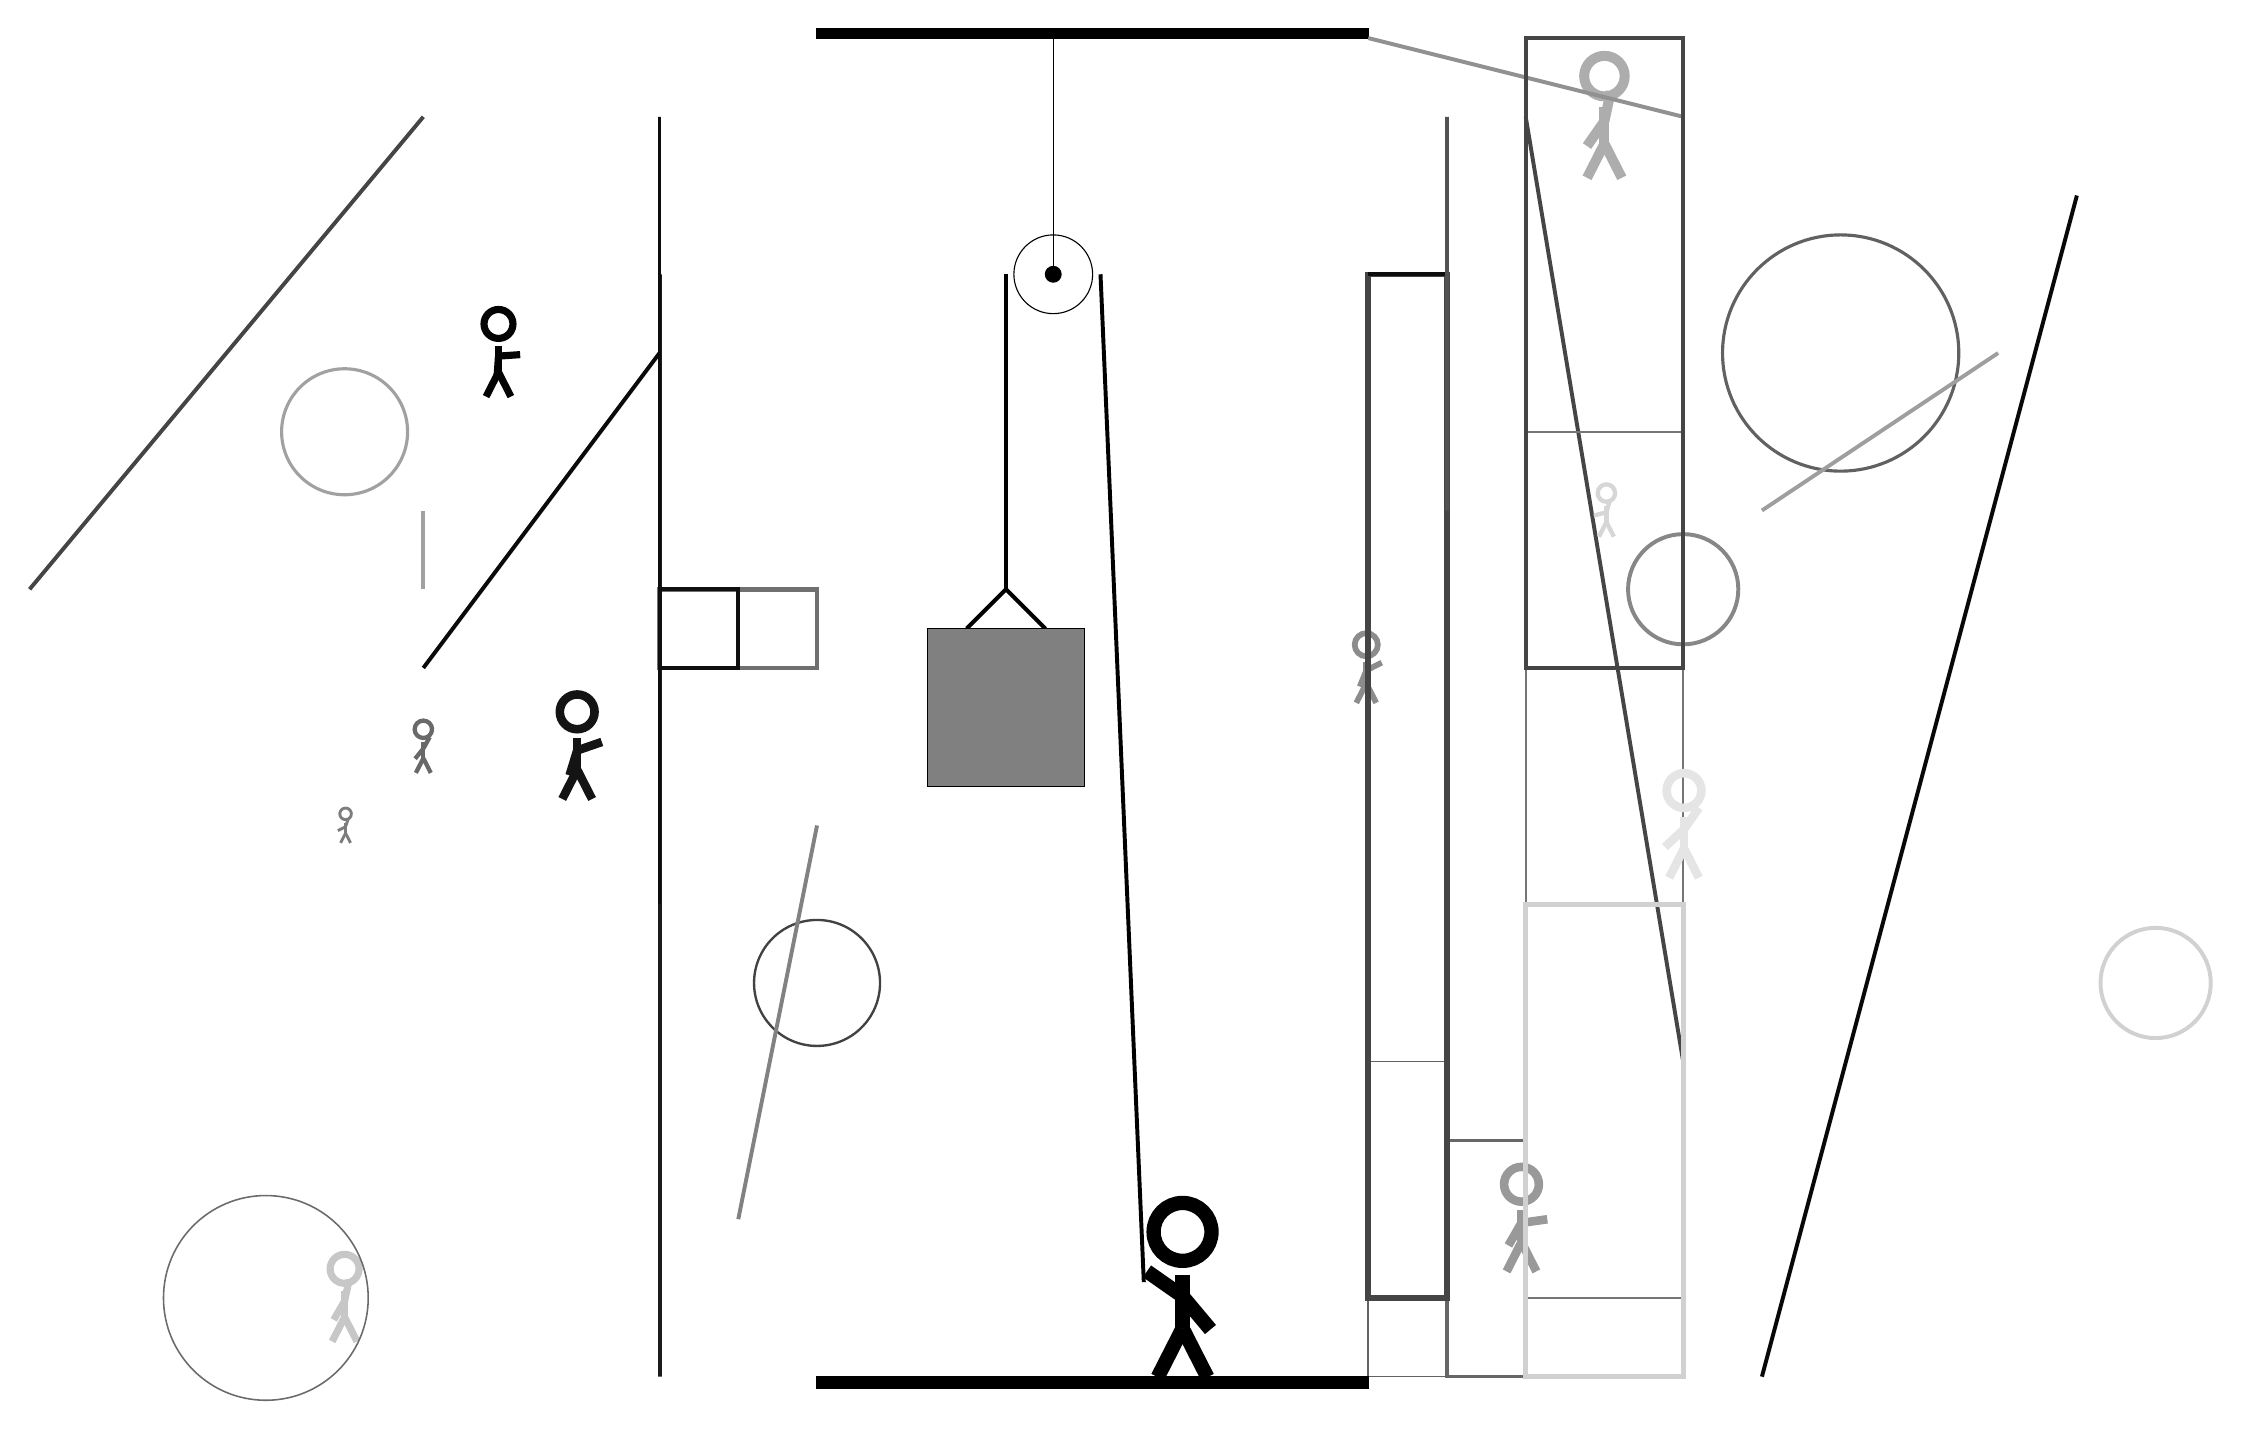
\begin{tikzpicture}
			%%%%% START %%%%%
			
			\draw[fill=black] (-2, 14) rectangle (5, 14.125);
			
			\draw (1, 11) circle (0.5);
			\draw[fill=black] (1, 11) circle (0.1);
			\draw (1, 14) -- (1, 11);
			
			\draw[line width=0.5mm] (-0.1, 6.5) -- (0.4, 7.0) -- (0.9, 6.5);
			\draw[fill=black!50] (-0.6, 6.5) rectangle (1.4, 4.5);
			
			\draw [line width=0.4mm, color=black!62](11, 10) circle (1.5);
			
			\draw[line width=0.5mm, color=black!89] (-4, 11) rectangle (-4, -3);
			\draw[line width=0.6mm, color=black!56] (-2, 7) rectangle (-4, 6);
			\node[line width=0.3mm, color=black!40] at (7, -1) {\Strichmaxerl[6][60][8]};
			
			\draw [line width=0.3mm, color=black!74](-2, 2) circle (0.8);
			\node[line width=0.3mm, color=black!32] at (8, 13) {\Strichmaxerl[7][55][78]};
			\draw[line width=0.5mm, color=black!73](7, 13) -- (9, 1);
			\draw[line width=0.2mm, color=black!61] (5, 1) rectangle (6, -3);
			\node[line width=0.6mm, color=black!22] at (-8, -2) {\Strichmaxerl[5][60][78]};
			\draw [line width=0.2mm, color=black!58](-9, -2) circle (1.3);
			\node[line width=0.2mm, color=black!45] at (5, 6) {\Strichmaxerl[4][68][27]};
			\draw[line width=0.5mm, color=black!73](-7, 13) -- (-12, 7);
			\node[line width=0.6mm, color=black!92] at (-5, 5) {\Strichmaxerl[6][73][19]};
			\draw[line width=0.4mm, color=black!60] (7, 0) rectangle (6, -3);
			\draw[line width=0.3mm, color=black!54] (7, -2) rectangle (9, 9);
			\draw [line width=0.5mm, color=black!18](15, 2) circle (0.7);
			
			\draw[line width=0.3mm, color=black!95] (-4, 13) rectangle (-4, 3);
			\draw[line width=0.5mm, color=black!97](10, -3) -- (14, 12);
			\draw[line width=0.7mm, color=black!73] (6, 11) rectangle (5, -2);
			
			\node[line width=0.4mm, color=black!16] at (8, 8) {\Strichmaxerl[3][14][74]};
			\draw[line width=0.5mm, color=black!95](5, 11) -- (6, 11);
			
			\draw [line width=0.4mm, color=black!37](-8, 9) circle (0.8);
			\draw[line width=0.5mm, color=black!96](-4, 10) -- (-7, 6);
			\draw[line width=0.5mm, color=black!37](-7, 7) -- (-7, 8);
			\draw[line width=0.5mm, color=black!94] (-3, 6) rectangle (-4, 7);
			
			\node[line width=0.6mm, color=black!59] at (-7, 5) {\Strichmaxerl[3][51][61]};
			\node[line width=0.7mm, color=black!99] at (-6, 10) {\Strichmaxerl[5][86][4]};
			\draw[line width=0.5mm, color=black!43](9, 13) -- (5, 14);
			\draw[line width=0.5mm, color=black!49](-2, 4) -- (-3, -1);
			
			\draw [line width=0.5mm, color=black!47](9, 7) circle (0.7);
			\draw[line width=0.7mm, color=black!66] (7, 14) rectangle (7, 14);
			\draw[line width=0.5mm, color=black!73] (7, 6) rectangle (9, 14);
			\node[line width=0.6mm, color=black!51] at (-8, 4) {\Strichmaxerl[2][27][71]};
			\draw[line width=0.5mm, color=black!38](10, 8) -- (13, 10);
			\draw[line width=0.6mm, color=black!18] (7, 3) rectangle (9, -3);
			\draw[line width=0.5mm, color=black!68] (6, 8) rectangle (6, 13);
			\node[line width=0.4mm, color=black!10] at (9, 4) {\Strichmaxerl[6][43][55]};
			
			
			\draw[line width=0.5mm] (0.4, 11) -- (0.4, 7.0);
			\centerarc[line width=0.5mm](1, 11)(0:180:0.6);
			\draw[line width=0.5mm](1.6, 11) -- (2.15, -1.8);
			
			\node at (2.6, -1.9) {\Strichmaxerl[10][-35][-50]};
			
			\draw[fill=black] (-2, -3) rectangle (5, -3.15);
			
			%%%%% END %%%%%
		\end{tikzpicture}
	\end{figure}	
\end{document}